\section{Machine Vision }

The vision subsystem is a critical component of AquaTux because it is
the one performing the identification of mission objectives. It is
also complementary to the passive sonar to grab the suitcase above the
acoustic pinger. Because the turbidity of the water and the small
number of visual features in the underwater floor prevent making
reliable correspondences between two views, we decided that stereo
vision was impractical in our vessel. Instead, we use two independent
cameras: one facing forward and one facing down. Since they
are rigidly attached to the AUV, we need to move the AUV
to change the viewpoint. In this section, we explain in more details
the features of our vision subsystem.


\subsection{Vision Hardware}
The vision hardware consists of two low light color cameras based
around $\frac{1}{3}$ inch Sony CCD sensors: these cameras were selected for their
image quality in low light situations, small size and price. Standard
adjustable lenses were used on each camera for maximum flexibility. A
Sensoray 311 capture card performs the video capture and frame
acquisition and communicates with our embedded computer through the
compact PC-104+ bus. The card provides 4 input channels at capture
rates up to 30 frames per second (fps). The computer does not sample
images at regular intervals: the actual frame rate depends on the
amount of processing required for a particular image, which will vary
depending on the task. The on-board computer was chosen to ensure that
it is fast enough to achieve a processing frame rate of at least 10
fps.  While we initially selected a Blackfin DSP to do the task, we
later decided to upgrade to a full-featured embedded Pentium 4 1.8Ghz
computer. This computer is equipped with an Ethernet port allowing to
connect to the wireless tether.


\subsection{Software Organization}
\label{gui}


\begin{figure}
\begin{center}
 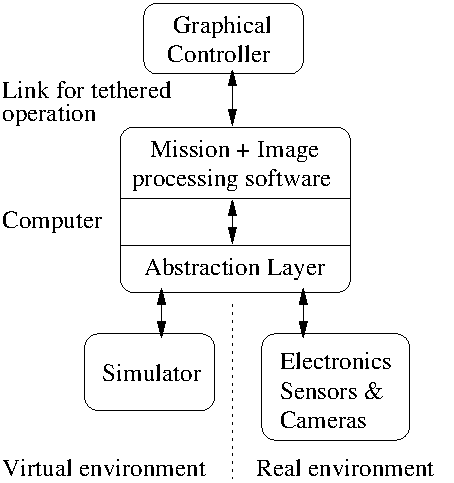
\includegraphics[width=2.2in]{fig/vision}
\caption{Vision modules organization in the AUV.}\label{vision}
\end{center}
\end{figure}


\begin{figure}
\begin{center}
 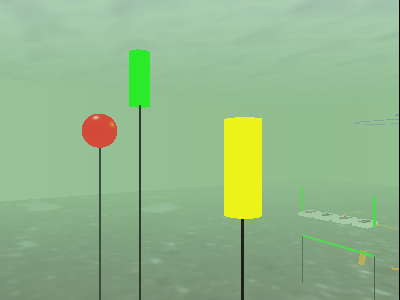
\includegraphics[width=2.7in]{fig/sim}
\caption{Example image from the simulator showing pipe segments, a box
  and a red buoy in turbid water.}\label{sim}
\end{center}
\end{figure}

The vision system is broken down in 3
software components (Figure~\ref{vision}): (i) the mission software that performs the image
processing; (ii) the simulator that recreates synthetic underwater
images based on the vehicle position (example in
Figure~\ref{sim}) and (iii) the graphical interface that is used to
control the mission software. The simulator and the graphical
interface were solely created to test and debug the vision
algorithms when AquaTux is not functioning autonomously. All modules connect through TCP/IP in a
very flexible and extensible fashion. This allows us to seamlessly
replace the simulator by the real hardware sensors and electronics
when we take our system from the lab to the water environment. The
graphical interface allows us to access all the data structures in the
AUV and can act as a passive observer, constantly requesting the
state of the vehicle, or as a controller sending commands to the
vessel.



\vspace{-.1in}
\subsection{Image Processing Software}
The image processing software consists of color filters and edge and
line detection algorithms. The color filters allow us to select
specific information to only process relevant parts of the images. The
line processing algorithms use heuristics to form polygons and
recognize objects such as pipes or boxes, that have a well defined
appearance. Our algorithms are robust enough to recognize objects even
if their view changes due to perspective or the presence of debris in
the water.  The mission software consists of a main loop that acquires
images, processes them and send commands to the other subsystems on
one of the two serial ports of the embedded computer (see
Section~\ref{gui}). The mission is broken down into modular tasks that
can me chained or tested individually. Tasks proceed by first
identifying a target for the vehicle to begin pursuit. If the object
in question is not found, the vehicle rotates on its vertical axis
(yaw) to make the cameras pan to the right and to the left. If nothing
is found, then the vehicle proceeds forward in its initial direction.
Once a target is acquired, the vertical position and lateral positions
of the vessel are controlled to match the desired coordinates.  The
vehicle uses a combination of heading relative to its current
orientation and absolute headings (relative to the magnetic north
pole) to navigate inside the environment. This alleviates the need to
get real-time measurements of the heading as the vehicle is
navigating. A limitation of our vision hardware that we had to address
is to determine when a task is completed if the view of the target is
obscured or occluded due to the AUV's proximity (e.g. it is passing
under the gate). In such situations, for the moment being, we use
timers to ensure that the vehicle reaches its target location.
